%===================================== CHAP 2 =================================

\chapter{Background}

\section{NAV}
NAV is currently funding a pilot project in partnership with the IMTEL lab at NTNU investigating different XR technologies and attempting to determine their viability in helping those receiving support from NAV to find employment. As part of this, NAV and IMTEL has collaborated to create several workplace experiences to introduce new working environments to potential employees in a safe and educational environment.

This thesis and underlying project is a part of this, and can be considered a branch project. While normal development continues on workplaces, this project attempt to research the effects that multi-user experiences have on the learning efficacy of the users attempting to find employment through NAV's programs.

%Nyttig link :) https://www.nrk.no/vestfold/nytt-pilotprosjekt_-gaming-hjelper-johan-_22_-a-velge-riktig-yrke-1.14748067


\section{Concepts}
This section explains some of the essential concepts for this thesis.


\subsection{Reality-Virtuality Continuum} \label{background:Continuum}
In 1996, Paul Milgram described the \textit{Reality-Virtuality Continuum}\cite{milgram1995augmented}. The paper describes in detail the different types of virtuality and reality that exist on this scale, and the major differences that separate them. As Figure \ref{fig:VR_continuum} illustrates the the real world and virtual world are opposite ends of the continuum, with mixed reality (MR) covering the majority, but not including, the fully real and virtual environments. 

The applications developed for NAV during this project find themselves at the right hand side of the continuum, as mostly virtual environments, but also within the mixed reality concept.  

\begin{figure}
    \centering
    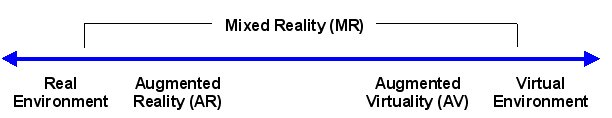
\includegraphics[width=\textwidth]{./fig/background/Virtuality_Continuum_2}
    \caption{The Virtuality-Reality Continuum}
    \label{fig:VR_continuum}
\end{figure}


\subsubsection{Virtual Reality}
The definition of virtual reality has changed over the years, for example when Milgram et al. defined it 1995 \cite{milgram1995augmented} as an environment in which "...participant-observer is totally immersed in a completely synthetic world, which may or may not mimic the properties of a real-world environment, either existing or fictional, but which may also exceed the bounds of physical reality by creating a world in which the physical laws governing gravity, time and material properties no longer hold." D. Guttentag \cite{guttentag2010virtual} later defined it in 2010 as “the use of a computer-generated 3D environment...that one can navigate and possibly interact with, resulting in real-time simulation...".

Although definitions differ, the concept remains the same - a virtual environment which supports navigation and interaction. Today, these environments are often displayed to the user using a head mounted display (HMD), but there exists other ways, including room scale projections.

\subsubsection{Mixed Reality} \label{background:MixedReality}
As with virtual reality, the definition of mixed reality (MR) has changed from when Milgram et al. defined it  \cite{milgram1995augmented} as an environment where "...real world and virtual world object are presented together within a single display...". It can been seen as anywhere on the continuum except on the extrema, see Figure \ref{fig:VR_continuum}. However, the usage of the term MR has been somewhat lose with manufactures such as HP and Microsoft putting it on their headsets or in their desktop application. In the \textit{What is mixed reality?} \cite{microsoftMR} article by Microsoft they describe it as a blend of physical and digital world where the mixed reality spectrum covers and fully includes the physical world and the digital world, unlike the continuum by Milgram et al. which does not, see Figure \ref{fig:MicrosoftSpectrum}.

Although, they are quite similar it is important to note and that for this project we will follow the definition of MR defined by Milgram et al., which means whenever we refer to mixed reality we do not include the fully real- or virtual environment in that reasoning.  

\begin{figure}
    \centering
    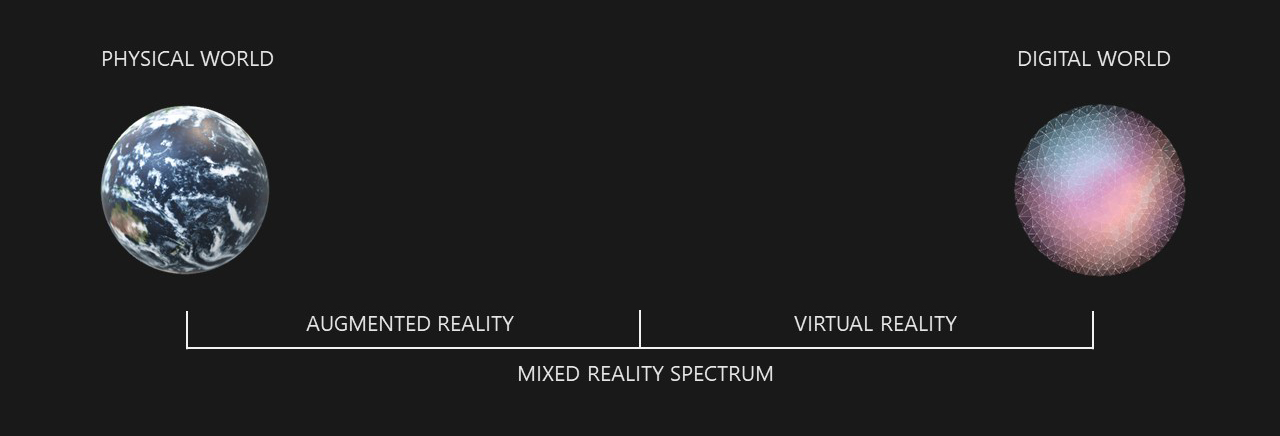
\includegraphics[width=\textwidth]{./fig/background/microsoft_spectrum.jpg}
    \caption{The mixed reality spectrum according to Microsoft \cite{microsoftMR}.}
    \label{fig:MicrosoftSpectrum}
\end{figure}


  
\subsection{Immersion and presence} \label{immersionAndPresence}
It's important to note the difference between presence and immersion. While immersion refers to an an objective level of fidelity, which can be measured against the immersion levels of another application, presence refers to a person's subjective feeling of being in a location while physically being in another \cite{slater2003note}. With this project we hope to increase the presence of the user in the virtual workplaces, not necessarily the immersion.

\subsection{Workspace Awareness in Groupware}
When collaborating with others, there are several ways in which we gather information. Many of these are subtle and perhaps not outright obvious, but are important none the less as ways to collaborate efficiently. The awareness of others' location, actions and intentions in regard to the task are referred to as \textit{workspace awareness}.

When working with groupware, workspace awareness is not a given. It must be implemented by developers and rigorously tested to make sure it works well. The developer must explicitly create the forms of interaction and tools to support workspace awareness\cite{gutwin1996workspace}.

In spite of this, one does not need to start entirely from a blank sheet. There are certain elements that make up the core elements of workspace awareness, as seen in tables \ref{table:awarenessPresent} and \ref{table:awarenessPast}\cite{gutwin2002descriptive}. Using these categories as a framework, one can more easily consider what parts are necessary for the workspace you are creating and make decisions based on that.

\begin{table}[!h]

      \centering
        \caption{Elements of workspace awareness relating to the present}
        \begin{tabularx}{\textwidth}{lll}
        \toprule
        Category & Element & Specific Questions\\
        \midrule
        Who & Presence & Is anyone in the workspace?\\
         & Identity & Who is participating? Who is that?\\
        \vspace{0.2cm}
         & Authorship & Who is doing that?\\
        
        What & Action & What are they doing?\\
         & Intention & What goal is that action part of?\\
        \vspace{0.2cm}
         & Artifact & What object are they working on?\\
        
        Where & Location & Where are they working?\\
         & Gaze & Where are they looking?\\
         & View & Where can they see?\\
         & Reach & Where can they reach?\\
        
        \bottomrule
        \label{table:awarenessPresent}
        \end{tabularx}
\end{table}

\begin{table}[!h]
      \centering
        \caption{Elements of workspace awareness relating to the past}
        \begin{tabularx}{\textwidth}{lll}
        \toprule
        Category & Element & Specific Questions\\
        \midrule
        How & Action history & How did that operation happen?\\
        \vspace{0.2cm}
         & Artifact history & How did this artifact come to be in this state?\\\vspace{0.2cm}
        When & Event history & When did that event happen?\\\vspace{0.2cm}
        Who (past) & Presence history & Who was here, and when?\\\vspace{0.2cm}
        Where (past) & Location history & Where has a person been?\\\vspace{0.2cm}
        What (past) & Action history & What has a person been doing?\\
        \bottomrule
        \label{table:awarenessPast}
        \end{tabularx}
\end{table}

In the versions of the applications made for one user at a time, the guidance counsellor/operator would have to explain how things like tasks worked and where objectives were located without existing in the same virtual space. This disconnect proved disadvantageous and ineffective, and the presence of the user suffered due to the disconnect between the virtual space they were in and the instructions coming in from outside of this space. Enabling workspace awareness with others, be it other users or supervisors, enhances several activities. A brief summary of these can be seen in table \ref{table:awarenessActivity} \cite{gutwin2002descriptive}. Several of these activities can be strongly enhanced with the introduction of groupware, particularly with VR. While all of these are important, a few of them are more relevant than the others.

\begin{table}[!h]
      \centering
        \caption{Summary of the activities in which workspace awareness is used}
        \begin{tabularx}{\textwidth}{l X}
        \toprule
        Activity & Benefit of workspace awareness \\
        \midrule
        Management of coupling & Assists people in noticing and managing transitions between individual and shared work.\\
        \vspace{0.2cm}
        Simplification of communication & Allows people to the use of the workspace and artifacts as conversational props, including mechanisms of deixis, demonstrations, and visual evidence.\\\vspace{0.2cm}
        Coordination of action & Assists people in planning and executing low-level workspace actions to mesh seamlessly with others.\\\vspace{0.2cm}
        Anticipation & Allows people to predict others’ actions and activity at several time scales.\\\vspace{0.2cm}
        Assistance & Assists people in understanding the context where help is to be provided.\\
        \bottomrule
        \label{table:awarenessActivity}
        \end{tabularx}
\end{table}

\subsection{Tutoring}
For those struggling to enter the workforce, it is important that they are able to get the proper impression of a workplace. If more time is spent failing certain tasks rather then organically exploring the tasks at hand, the participant may be discouraged from trying more. Having a tutor or another similar figure present to help keep them on track can be quite beneficial as long as they follow some basic tutoring principles, according to a study by Douglas C. Merill in 1995 \cite{merrill1995tutoring}.

\subsection{Computer-Supported Collaborative Learning} \label{CSCL}
\label{section:CSCL}
The field of CSCL is highly relevant to the task at hand. CSCL is a multi-disciplinary field seeking to use technology to empower users to collaborate and learn together \cite{stahl2006computer}.  It's also important to make the distinction between \textit{collaboration} and \textit{cooperation}. Where as cooperation is defined by Dillenbourg as the division of work into subtasks which eventually are pieced together to form a final result, he defines collaboration as working "together" \cite{dillenbourg1999you}.

The concept can roughly be split into two parts. Namely, the computer support and the collaborative learning. CSCL is inherently social, and the technology must strive to support that. Technology also offers unique opportunities that need to be catered to, rather than attempting to create something that does not take advantage of these opportunities, or tries to solve problems for which the technology is not suited.

The collaborative learning aspect is interesting because not only do you use collaboration to increase the learning effect, the learning itself is constituted of the interaction between the participants\cite{stahl2006computer}. That is to say, even should you attempt to learn something on your own, the knowledge you gain is inherently different from the knowledge one would gain through collaboration.


CSCL stresses collaboration among the users. When used properly, the users will learn together, motivate each other and gain a richer learning experience in general through collaborative learning.

%\subsection{Collaborative Virtual Environments for Supporting
%Learning Communities}
%Monica Divitini and Ekatarina paper 

\subsection{Education in VR}
A literature review in 2015 found that the uses for virtual reality in education were many, stating that "Immersive VR can offer great advantages for learning:  [...] it supports training in a safe environment avoiding potential real dangers and [...] it increases the learner's involvement and motivation..." \cite{freina2015literature}. While there are a general consent among the scientific community that virtual reality can contribute to educational efficacy there are some aspects to consider when developing VR applications for educational use. Roussos et al. describes several dimensions in relation to virtual reality and learning including \textit{technical}, \textit{orientation}, \textit{affective}, \textit{cognitive} and \textit{pedagogical} aspects \cite{roussos1999learning}, as seen in Table \ref{table:awarenessAspects}.

\begin{table}[!h]
      \centering
        \caption{Summary of the aspects defined by Roussos et al. \cite{roussos1999learning} }
        \begin{tabularx}{\textwidth}{l X}
        \toprule
        Aspect \hspace{1.5cm} & Description \\
        \midrule
        Technical & Usability regarding the interface, software and hardware.
        \vspace{0.2cm}
        \\
        Orientation & Navigation, spatial orientation, presence, immersion and feedback. 
        \vspace{0.2cm}
        \\
        Affective & User engagement, and confidence in the virtual environment.
        \vspace{0.2cm}
        \\
        Cognitive & Internal concepts through the users learning experience.
        \vspace{0.2cm}
        \\
        Pedagogical & Gain knowledge about the environment and concepts being thought.
        \vspace{0.2cm}
        \\
        \bottomrule
        \label{table:awarenessAspects}
        \end{tabularx}
\end{table}

\subsection{Gamification}
Gamification has been a common practice of enhancing a service by including game design principles in a non-game context in order to add value and thereby encourage the user to complete tasks which might seem less interesting on their own. A study by Hamari et al. \cite{hamari2014does} showed that the process yields positive effects and concludes that gamification does work. The IMTEL lab has used gamification principles in several of their projects as a mean to engage its users.   

\section{Technologies}
This section briefly explains some of the main technologies and frameworks that were used during the development of the applications. 

\subsection{Unity}
Unity is one of the most common game development engines used recently \cite{unity}. As this project builds an already established project, the same tools need to be used. Unity allows for quick editing of a scene, and provides a powerful toolset within its layers for developers. Scripting can be done with the C\# coding language when necessary, and it integrates well with numerous frameworks and plugins.

\subsection{OpenVR}
\textcolor{red}{Egen seksjon eller steamvr under openvr?}


\subsection{SteamVR}
SteamVR is an API distributed by Valve Corporation. It makes development for VR significantly easier, in that we only need to target the API, and it will make it work for all the major VR headset brands without any extra effort. It also handles input from headsets, and translating the controller input to a fully animated controller inside the application \cite{steamVR}\cite{steamVRAPI}.

\subsection{PUN2 - Photon Networking}
Photon is a multiplayer framework that enables fast and easy setup of a multiplayer server and matchmaking. Specifically, their own wrapper of the framework for Unity, Photon Unity Networking (or PUN) can be imported directly into a Unity project and work seamlessly from there with minimal coding required to function. While the base level of functionality is quite simple, some more work is required to make it fit certain applications \cite{PUN}.

\subsection{Git}
Git is a version-control-system for collaborative software development work. It makes it easy for multiple participants to work together on single project, and abstracts away a lot of the work involved in merging multiple pieces of code together. For this project we used GitLab \cite{GitLab} as Git-repository manager since the IMTEL lab has their own codebase there.


\subsection{Head-mounted displays}
For this project we use SteamVR API and are therefore not limited to the development of software for specific head-mounted displays (HMDs). The IMTEL lab offers several modern HMDs including HTC Vive Pro, Valve Index, HP Reverb Mixed Reality and numerous Oculus headsets. The main difference between these HMDs is the use of "base stations" - wall mounted tracking sensors. HTC Vive Pro (seen in Figure \ref{fig:htcVivePro}) uses these sensors, whereas the HP Reverb (seen in Figure \ref{fig:hpReverb}) does not. Instead it tracks controllers and position using built in sensors in the headset. This is useful when performing test outside the IMTEL lab as there is no need to use base stations.   

\begin{figure}
    \centering
    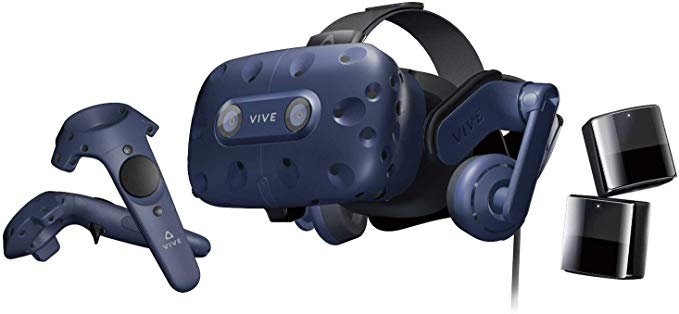
\includegraphics[width=0.65\textwidth]{./fig/background/htcVivePro.jpg}
    \caption{HTC Vive Pro with controllers and base stations.}
    \label{fig:htcVivePro}
\end{figure}

\begin{figure}
    \centering
    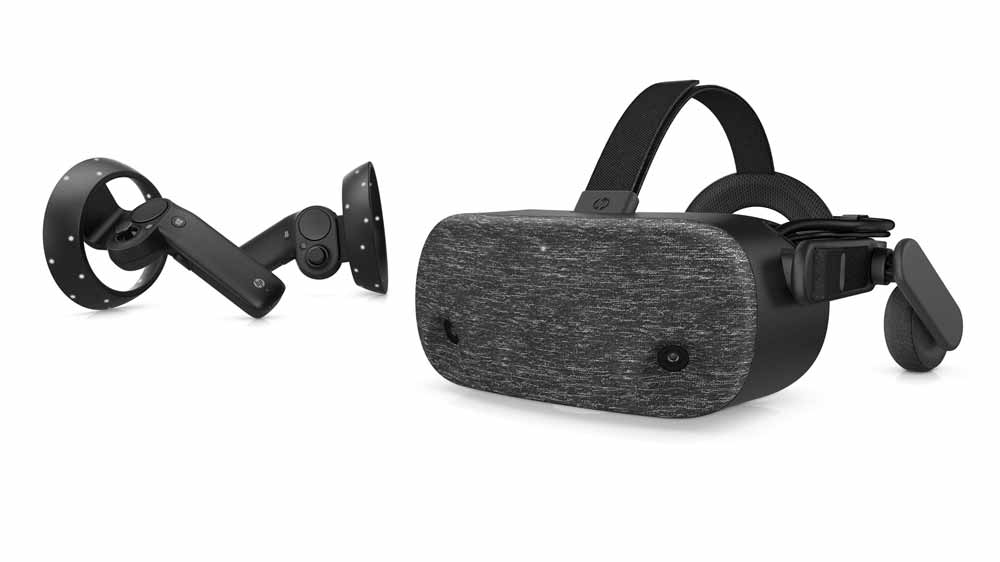
\includegraphics[width=0.65\textwidth]{./fig/background/hpReverbPro.jpg}
    \caption{HP Reverb Mixed Reality with controllers.}
    \label{fig:hpReverb}
\end{figure}

\cleardoublepage